\doublespacing % Do not change - required

\chapter{Introduction}
\label{ch1}

%%%%%%%%%%%%%%%%%%%%%%%%%%%%%%%%%%%%%%%
% IMPORTANT
\begin{spacing}{1} %THESE FOUR
\minitoc % LINES MUST APPEAR IN
\end{spacing} % EVERY
\thesisspacing % CHAPTER
% COPY THEM IN ANY NEW CHAPTER
%%%%%%%%%%%%%%%%%%%%%%%%%%%%%%%%%%%%%%%

The accurate forecasting of implied volatility surfaces represents one of the most challenging and practically important problems in quantitative finance. These surfaces encode market expectations of future uncertainty across option strikes and maturities, serving as fundamental inputs to derivatives pricing, portfolio hedging, and risk management systems. However, the high-dimensional, structured nature of implied volatility data, combined with strict no-arbitrage constraints, renders conventional forecasting approaches inadequate. This project develops and evaluates neural network-based forecasting models that explicitly account for the multi-dimensional structure of implied volatility surfaces while ensuring financial consistency through the use of arbitrage-free parametric representations.

\section{Options, Risk, and Implied Volatility}

Options are financial derivatives that confer the right, but not the obligation, to buy or sell an underlying asset at a predetermined strike price $K$ before or at a specified expiration date. The value of an option depends fundamentally on the uncertainty surrounding the future price of the underlying asset: greater uncertainty increases the probability of extreme outcomes, thereby enhancing the value of the optionality embedded in these contracts. This relationship between uncertainty and option value makes options natural instruments for both hedging against and speculating on future price volatility.

The Black--Scholes--Merton framework \cite{BlaSch:73,Mer:73} provides a foundational model for option pricing by assuming that asset prices follow geometric Brownian motion with constant volatility. Under this framework, the price of a European call option can be expressed in closed form, with volatility serving as the key parameter that summarises uncertainty about future price movements. However, when market prices of options are observed, inverting the Black--Scholes formula to solve for the volatility parameter that matches observed prices reveals a striking empirical regularity: implied volatility—the volatility level implied by market prices—varies systematically with both strike price and time to maturity, contradicting the constant-volatility assumption of the Black--Scholes model.

This systematic variation gives rise to the concept of an implied volatility surface: a function $\sigma_{\text{imp}}(K, \tau)$ that maps strike prices $K$ and times to maturity $\tau$ to their corresponding implied volatilities. The surface exhibits characteristic patterns: volatility smiles, where implied volatility is higher for out-of-the-money options than at-the-money options; volatility skews, where implied volatility is asymmetric around the at-the-money strike; and term structure effects, where implied volatility varies with maturity. These patterns reflect market perceptions of tail risk, jump risk, and the evolution of uncertainty over time, making the implied volatility surface a rich source of information about market expectations and risk preferences \cite{Gat:06,Fen:05}.

\section{Challenges in Forecasting Implied Volatility Surfaces}

The ability to accurately forecast implied volatility surfaces is of fundamental importance across quantitative finance. In derivatives pricing, surface forecasts enable the valuation of exotic options and structured products that depend on the joint behaviour of implied volatility across strikes and maturities. In hedging applications, accurate forecasts of how the surface will evolve are essential for dynamic hedging strategies that must adjust positions as market conditions change. In risk management, surface dynamics provide critical inputs for portfolio risk assessment, stress testing, and scenario analysis \cite{Gat:06}. Moreover, changes in the shape of the implied volatility surface reflect evolving market perceptions of tail risk, jump risk, and uncertainty \cite{Fen:05,ConTan:04}, making surface forecasting a key component of volatility trading and market-making strategies.

\subsection{High Dimensionality and Structured Dependencies}

From a statistical modelling perspective, implied volatility surfaces present a fundamentally high-dimensional forecasting problem. At each point in time, the surface is defined over a two-dimensional domain of strikes and maturities, typically discretised into hundreds or thousands of grid points. Forecasting therefore requires predicting the evolution of an entire surface-valued time series, rather than a scalar or low-dimensional vector. This high dimensionality is compounded by the fact that the surface exhibits rich cross-sectional structure: implied volatilities at neighbouring strikes and maturities are highly correlated, and changes in one region of the surface often propagate across others. When considered over time, this results in a three-way tensor with complex dependencies across strike, maturity, and temporal dimensions.

Naive approaches that flatten the surface into a high-dimensional vector discard this intrinsic structure, leading to several problems. First, the curse of dimensionality means that such models require enormous amounts of data to avoid overfitting. Second, the loss of structure makes it difficult to regularise models in a way that respects the geometry of volatility surfaces. Third, unstructured representations fail to exploit the fact that volatility surfaces exhibit smoothness and continuity across strikes and maturities, properties that can be naturally encoded in structured models \cite{Fen:05,Gat:06}. These limitations motivate the development of forecasting methods that explicitly preserve and exploit the multi-dimensional structure of implied volatility data.

\subsection{Data Quality and Estimation Stability}

Implied volatility surfaces are not directly observable but must be estimated from noisy market data. Option prices are subject to bid--ask spreads, liquidity effects, and market microstructure noise, all of which introduce measurement error into implied volatility estimates. This problem is particularly acute for short-dated options, deep out-of-the-money options, and options on less liquid underlyings, where pricing errors can translate into large fluctuations in implied volatility. The sensitivity of implied volatility to small changes in option prices—especially for options far from at-the-money—makes surface estimation and forecasting inherently unstable.

This instability poses a fundamental challenge for forecasting models. Models that are overly flexible risk fitting noise rather than meaningful structure, leading to poor out-of-sample performance. Conversely, models that are too rigid may fail to capture genuine surface dynamics. Achieving an appropriate balance between flexibility and stability requires careful regularisation and model design. Moreover, ensuring smoothness and continuity across both strike and maturity dimensions is essential for producing forecasts that are both statistically accurate and practically useful \cite{Fen:05,Gat:06}.

\subsection{Arbitrage-Free Constraints}

Beyond statistical considerations, implied volatility surfaces must satisfy fundamental no-arbitrage constraints that arise from the absence of static arbitrage opportunities in option markets. These constraints impose strict restrictions on the shape of the surface: for fixed maturity, call prices must be non-increasing and convex in strike; for fixed strike, call prices must be non-decreasing in maturity. Violations of these conditions would imply the existence of risk-free profit opportunities, which cannot persist in efficient markets.

Forecasts that violate no-arbitrage constraints are not only theoretically inconsistent but also practically problematic. Such forecasts may imply negative risk-neutral probabilities, lead to economically meaningless option prices, or produce unstable hedging ratios. Ensuring that forecasted surfaces satisfy these constraints is therefore a critical requirement for any forecasting model intended for use in pricing or hedging applications \cite{Gat:06,Fen:05}. However, incorporating such constraints into flexible, data-driven forecasting models is non-trivial. Parametric models can enforce constraints by construction, but at the cost of reduced flexibility. Non-parametric and machine learning approaches offer greater flexibility but face the challenge of ensuring that forecasts remain arbitrage-free, often requiring post-processing or constraint-aware training procedures.

\subsection{Existing Approaches and Their Limitations}

A wide range of approaches have been proposed for representing and forecasting implied volatility surfaces, each with distinct strengths and limitations. Parametric surface models, most notably those based on the stochastic volatility inspired (SVI) framework \cite{Gat:04} and its arbitrage-free extension, the surface SVI (SSVI) \cite{GatJac:14}, impose a low-dimensional parametric structure on the cross-section. These models can enforce no-arbitrage conditions by construction and offer interpretability through their parameters, which often have intuitive financial meanings. Forecasting within these frameworks typically proceeds through a two-step procedure: surface parameters are first estimated independently at each time point, and subsequently modelled dynamically using time-series techniques such as vector autoregression or state-space models \cite{Fen:05}. While such approaches offer stability and theoretical grounding, they rely on strong parametric assumptions that may be too restrictive to capture complex, non-linear, or regime-dependent surface dynamics.

More flexible statistical and machine learning approaches model implied volatility surfaces directly as discretised grids, treating the forecasting problem as a high-dimensional time-series prediction task. Recent work has explored neural network architectures, including long short-term memory (LSTM) networks \cite{AckTagVat:20}, variational autoencoders \cite{Bergeron:21}, and attention-based models, to capture complex temporal and cross-sectional dependencies. However, many of these approaches flatten the surface into a high-dimensional vector, discarding its inherent multi-dimensional structure and exacerbating the curse of dimensionality. Moreover, incorporating no-arbitrage constraints within such flexible frameworks remains challenging, often requiring constraint-aware loss functions or post-processing steps that may compromise forecast quality.

Recent work by Ackerer et al. \cite{AckTagVat:20} has demonstrated a promising hybrid approach that combines parametric SSVI surfaces with neural network correctors, working in total variance space to preserve arbitrage-free structure while allowing flexible corrections. This approach highlights the potential benefits of leveraging parametric models for structure and arbitrage-free guarantees while using neural networks for flexibility. However, the question of how best to forecast the evolution of such surfaces over time, particularly when working with parameter-based representations, remains an active area of research.

\section{Project Objectives and Methodology}

The primary objective of this project is to develop and evaluate neural network-based forecasting models for implied volatility surfaces that explicitly account for the multi-dimensional structure of volatility data while ensuring financial consistency through arbitrage-free representations. The project addresses the fundamental challenge of forecasting surface-valued time series by leveraging parametric surface models for structure and arbitrage-free guarantees, combined with neural network architectures for flexible temporal modelling.

\subsection{Methodological Approach}

The project adopts a two-stage methodology that combines the theoretical foundations of parametric volatility surface models with the flexibility of neural network forecasting. In the first stage, raw option market data are processed and interpolated using the surface stochastic volatility inspired (SSVI) framework \cite{GatJac:14}, which provides arbitrage-free surfaces in total variance space. This stage ensures that all surfaces used for forecasting satisfy no-arbitrage constraints by construction, addressing a critical limitation of approaches that work directly with raw implied volatility data.

In the second stage, the evolution of SSVI parameterised surfaces is forecasted using neural network architectures. Two complementary approaches are investigated: (1) direct forecasting of discretised surfaces on fixed grids, and (2) forecasting of SSVI parameters followed by surface reconstruction. The parameter-based approach offers several advantages: it operates in a low-dimensional space (typically 10--15 parameters per surface), naturally preserves arbitrage-free structure through SSVI reconstruction, and provides interpretability through parameter dynamics. Long short-term memory (LSTM) networks are employed to capture temporal dependencies in parameter evolution, with careful attention to parameter normalisation, constraint handling, and surface reconstruction.

\subsection{Evaluation Framework}

The performance of the proposed models is evaluated using comprehensive out-of-sample forecasting experiments on equity option data spanning multiple market regimes, including periods of normal volatility and extreme market stress. Forecasts are generated for multiple prediction horizons (1 day, 1 week, 1 month) and compared against baseline persistence models to assess the value added by the proposed approaches.

Evaluation metrics focus on implied volatility accuracy, as this is the most interpretable and widely used metric in both academic research and industry practice. The primary metric is root mean squared error in implied volatility space (IV RMSE), computed across all strikes and maturities. Secondary metrics include relative RMSE, mean absolute error, and maturity-specific and moneyness-specific error decompositions to identify regions where models perform well or poorly. All forecasts are validated to ensure they remain arbitrage-free, and qualitative assessments of surface smoothness and stability are conducted.

\subsection{Deliverables and Contributions}

The project delivers a fully implemented forecasting framework, including data processing pipelines, SSVI fitting and interpolation routines, neural network forecasting models, and comprehensive evaluation tools. The framework is designed to be modular and extensible, allowing for easy integration of additional models or datasets. Accompanying the implementation is a systematic empirical evaluation that compares the proposed approaches against baseline methods, identifies their strengths and limitations, and provides insights into the factors that drive forecasting performance.

The primary contributions of this work are: (1) a methodology that combines parametric surface models with neural network forecasting to achieve both flexibility and financial consistency; (2) an empirical evaluation that demonstrates the effectiveness of parameter-based forecasting for implied volatility surfaces; and (3) a critical analysis of the trade-offs between different forecasting approaches, providing guidance for practitioners on when and how to apply these methods. The project aims to advance the state of the art in volatility surface forecasting while maintaining the practical requirements of financial applications.


% \begin{figure}
% \centering
% 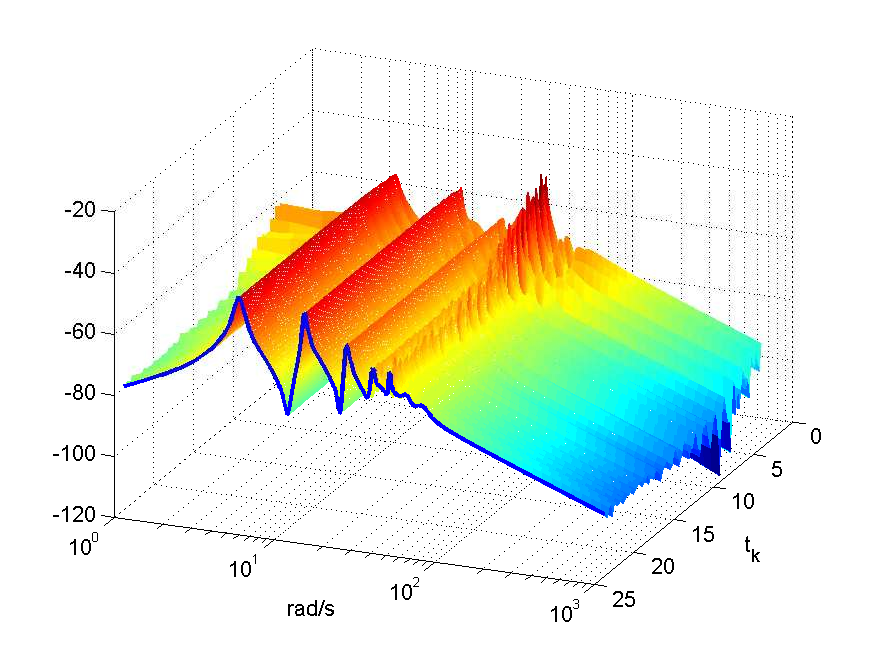
\includegraphics[width=0.8\columnwidth]{imgs/buildmagnitude.pdf}
% \caption[Short description for list of figures]{This figure is taken from \cite{Sca:16}.}
% \label{fig-magnitude}
% \end{figure}%




% \subsection{Title subsection}

% \kant[1-3]


% \section{Title section}

% \kant[1-5]

% \section{Notation}

% Standard notation has been adopted in the Thesis, most of which is defined in this section and used throughout the remainder of the Thesis. When new notation, not included in this section is introduced, this is defined in the relevant parts of the Thesis.\smallskip\\
% \indent The symbol $\mathbb{R}_{\ge0}$ ($\mathbb{R}_{>0}$) denotes the set of non-negative (positive) real numbers; $\mathbb{C}_{<0}$ denotes the set of complex numbers with strictly negative real part; $\mathbb{C}_{0}$ denotes the set of complex numbers with zero real part and $\mathbb{D}_{<1}$ the set of complex numbers with modulo less than one.\smallskip\\
% \indent The symbol $I$ denotes the identity matrix and $\sigma(A)$ denotes the spectrum of the matrix $A\in\mathbb{R}^{n\times n}$. The symbol $\otimes$ indicates the Kronecker product and $||A||$ indicates the induced Euclidean matrix norm. Given a list of $n$ elements $a_i$, $\diag(a_i)$ indicates a diagonal matrix with diagonal elements equal to the $a_i$'s. The vectorization of a matrix $A\in\mathbb{R}^{n\times m}$, denoted by $\vect(A)$, is the $nm \times 1$ vector obtained by stacking the columns of the matrix $A$ one on top of the other, namely $\vect(A)=[a_1^{\top},a_2^{\top},\dots,a_m^{\top}]^{\top}$, where $a_i\in\mathbb{R}^n$ are the columns of $A$ and the superscript $\top$ denotes the transposition operator. The superscript $*$ indicates the conjugate transpose operator.\smallskip\\
% \indent The symbol $\Re[z]$ indicates the real part of the complex number $z$, $\Im[z]$ denotes its imaginary part and $\iota$ denotes the imaginary unit. The symbol $\epsilon_k$ indicates a vector with the $k$-th element equal to 1 and with all the other elements equal to 0. Given a function $f$, $\overline{F}$ represents its phasor at $\omega$, whereas $<\!f(t)\!>$ indicates its time average.\smallskip\\
% \indent Given a set of delays $\{\tau_j\}$, the symbol $\mathfrak{R}_T^n=\mathfrak{R}_T^n([-T,0],\mathbb{R}^n)$, with $T=  \max_j\{\tau_j\}$, indicates the set of continuous functions mapping the interval $[-T,0]$ into $\mathbb{R}^n$ with the topology of uniform convergence . The subscripts ``$\tau_j$'' and ``$\chi_j$'' denote the translation operator, \textit{e.g.}\ $x_{\tau_j}(t)=x(t-\tau_j)$.\smallskip\\
% \indent Let $\bar s \in \mathbb{C}$ and $A(s)\in \mathbb{C}^{n \times n}$. Then $\bar s\notin\sigma(A(s))$ means that $\det(\bar s I-A(\bar s ))\ne0$. $\sigma(A(s))\subset\mathbb{C}_{<0}$ means that for all $\bar s$ such that $\det(\bar s I-A(\bar s ))=0$, $\bar s \in\mathbb{C}_{<0}$.\smallskip\\
% \indent The symbol $\mathcal{L}(f(t))$ denotes the Laplace transform of the function $f(t)$ (provided that $f(t)$ is Laplace transformable) and $\mathcal{L}^{-1}\{F(s)\}$ denotes the inverse Laplace transform of $F(s)$ (provided it exists). With some abuse of notation, $\sigma(\mathcal{L}(f(t)))$ denotes the set of poles of $\mathcal{L}(f(t))$. Given two functions, $f:Y\to Z$ and $g:X\to Y$, with $f\,\circ\,g:X\to Z$ we denote the composite function $(f\,\circ\,g)(x)=f(g(x))$ which maps all $x\in X$ to $f(g(x))\in Z$.


% \section{Published material}

% \kant[1]
